\documentclass[12pt,a4paper]{article}
\usepackage{subcaption}
\usepackage[utf8]{inputenc}
\usepackage[T1]{fontenc}
\usepackage{amsmath}
%\usepackage{mathaccent}
\usepackage{amsfonts}
\usepackage{amssymb}
\usepackage{makeidx}
\usepackage{graphicx}
\usepackage{float}
\usepackage{mathtools}
\usepackage{wrapfig}
\usepackage{ragged2e}
\usepackage{gensymb} 
\usepackage{fancyhdr}
\usepackage{fancybox}
\usepackage{natbib}
\usepackage[export]{adjustbox}
\usepackage[french]{babel}
\usepackage{pdfpages}
\usepackage{supertabular}
\usepackage{tabu}
\usepackage{array}
\usepackage{url}
\usepackage{enumitem}
\usepackage{subcaption}
\usepackage{caption}
\captionsetup{justification=raggedright,singlelinecheck = false}
\usepackage{multicol}
\usepackage{newcent}
\usepackage{environ}
\usepackage{emptypage}
\usepackage{makecell}

%%%%%%%%%%%%%%%%%%%%%%%%%%%%%%%%%%%%%%%%%%%%%%


%%%%%%%%%%%%ndex%%%%%%%%%%%%%%%%%%%%%%%%%%%%%%%%%%%%%%%%%%
\NewEnviron{myequation}{%
\begin{equation}
\scalebox{1.5}{$\BODY$}
\end{equation}
}
% \usepackage[backend=biber,bibencoding=utf8,style=verbose-inote,citestyle=authortitle]{\usepackage{xpatch}
% \usepackage{xpatch}
% 

\setlength{\arrayrulewidth}{0.7mm}
\setlength{\tabcolsep}{8pt}
\renewcommand{\arraystretch}{1}
% \usepackage{gfsartemisia}


% Changement de style de fonts pour la règlementation %%%
\newcommand*{\myfont}{\fontfamily{phv,9pt}\selectfont}

%Création de l'environnement pour les équations à description%
\newenvironment{conditions}
  {\par\vspace{\abovedisplayskip}\noindent\begin{tabular}{>{$}l<{$} @{${}={}$} 
l}}
  {\end{tabular}\par\vspace{\belowdisplayskip}}

\usepackage[left=1.80cm, right=1.90cm, top=2cm, bottom=2cm]{geometry}


\author{Cyrille Reggio}
\title{Moteurs gaz}
% \date{\today}
% \make
\makeindex



 \fancyhf{}
 \fancyhead[R]{\leftmark}
\lhead{ENSM}
\rhead{2017}
\chead{\textbf{Simulateur DFDE}}
\cfoot{\thepage}
 %%%%%%%%%%%%%%%%%%%%%%%%%%%%%%%%%%%%%
%Image simple : \image{url}{légende}{scale}
 \newcommand{\image}[3]
 {\begin{figure}[H]
         \begin{center}
          \includegraphics[width=#3\textwidth]{img/#1}
          \caption{#2} \label{img_#1}
         \end{center}
  \end{figure}
}

%%%%%%%%%%%%%%%%%%%%%%%%%%%%%
\newcommand{\gui}[1]
{\og #1 \fg~}
%%%%%%%%%%%%%%%%%%%%%%%%%%%%%
%Image cote à cote 
\newcommand{\imcac}[3]
{
\begin{figure}[h]
 
    \begin{subfigure}{0.5\linewidth}
        \centering
        \includegraphics[scale=#3,left]{img/#1}
    \end{subfigure}
    \begin{subfigure}{0.5\linewidth}
        \centering
        \includegraphics[scale=#3,right]{img/#2}
        %\caption{}
    \end{subfigure}

\end{figure}
}
%%%%%%%%%%%%%%%%%%%%%%%%%%%%%%%%%
\begin{document}

\thispagestyle{empty}
\pagenumbering{gobble}% Remove page numbers (and reset to 1)
\begin{minipage}{0.45\textwidth}
	\begin{figure}[H]
		
\includegraphics[scale=0.6]{img/ensm-logo.eps}
	\end{figure}
\end{minipage}

\begin{minipage}{0.9\textwidth}
	\flushright{\huge{Kongsberg}\\
	\huge{Dual-Fuel Diesel Electri}\\
	   % \huge{Moteurs gaz}\\
    \large{Procedure}}
       % \large{Sécurité de l'installation}\\
       % \large{Émissions et cycles}\\
       % \large{Applications aux moteurs}}
\end{minipage}						

\vfill
			
			\begin{figure}[hbtp]
			\centering
			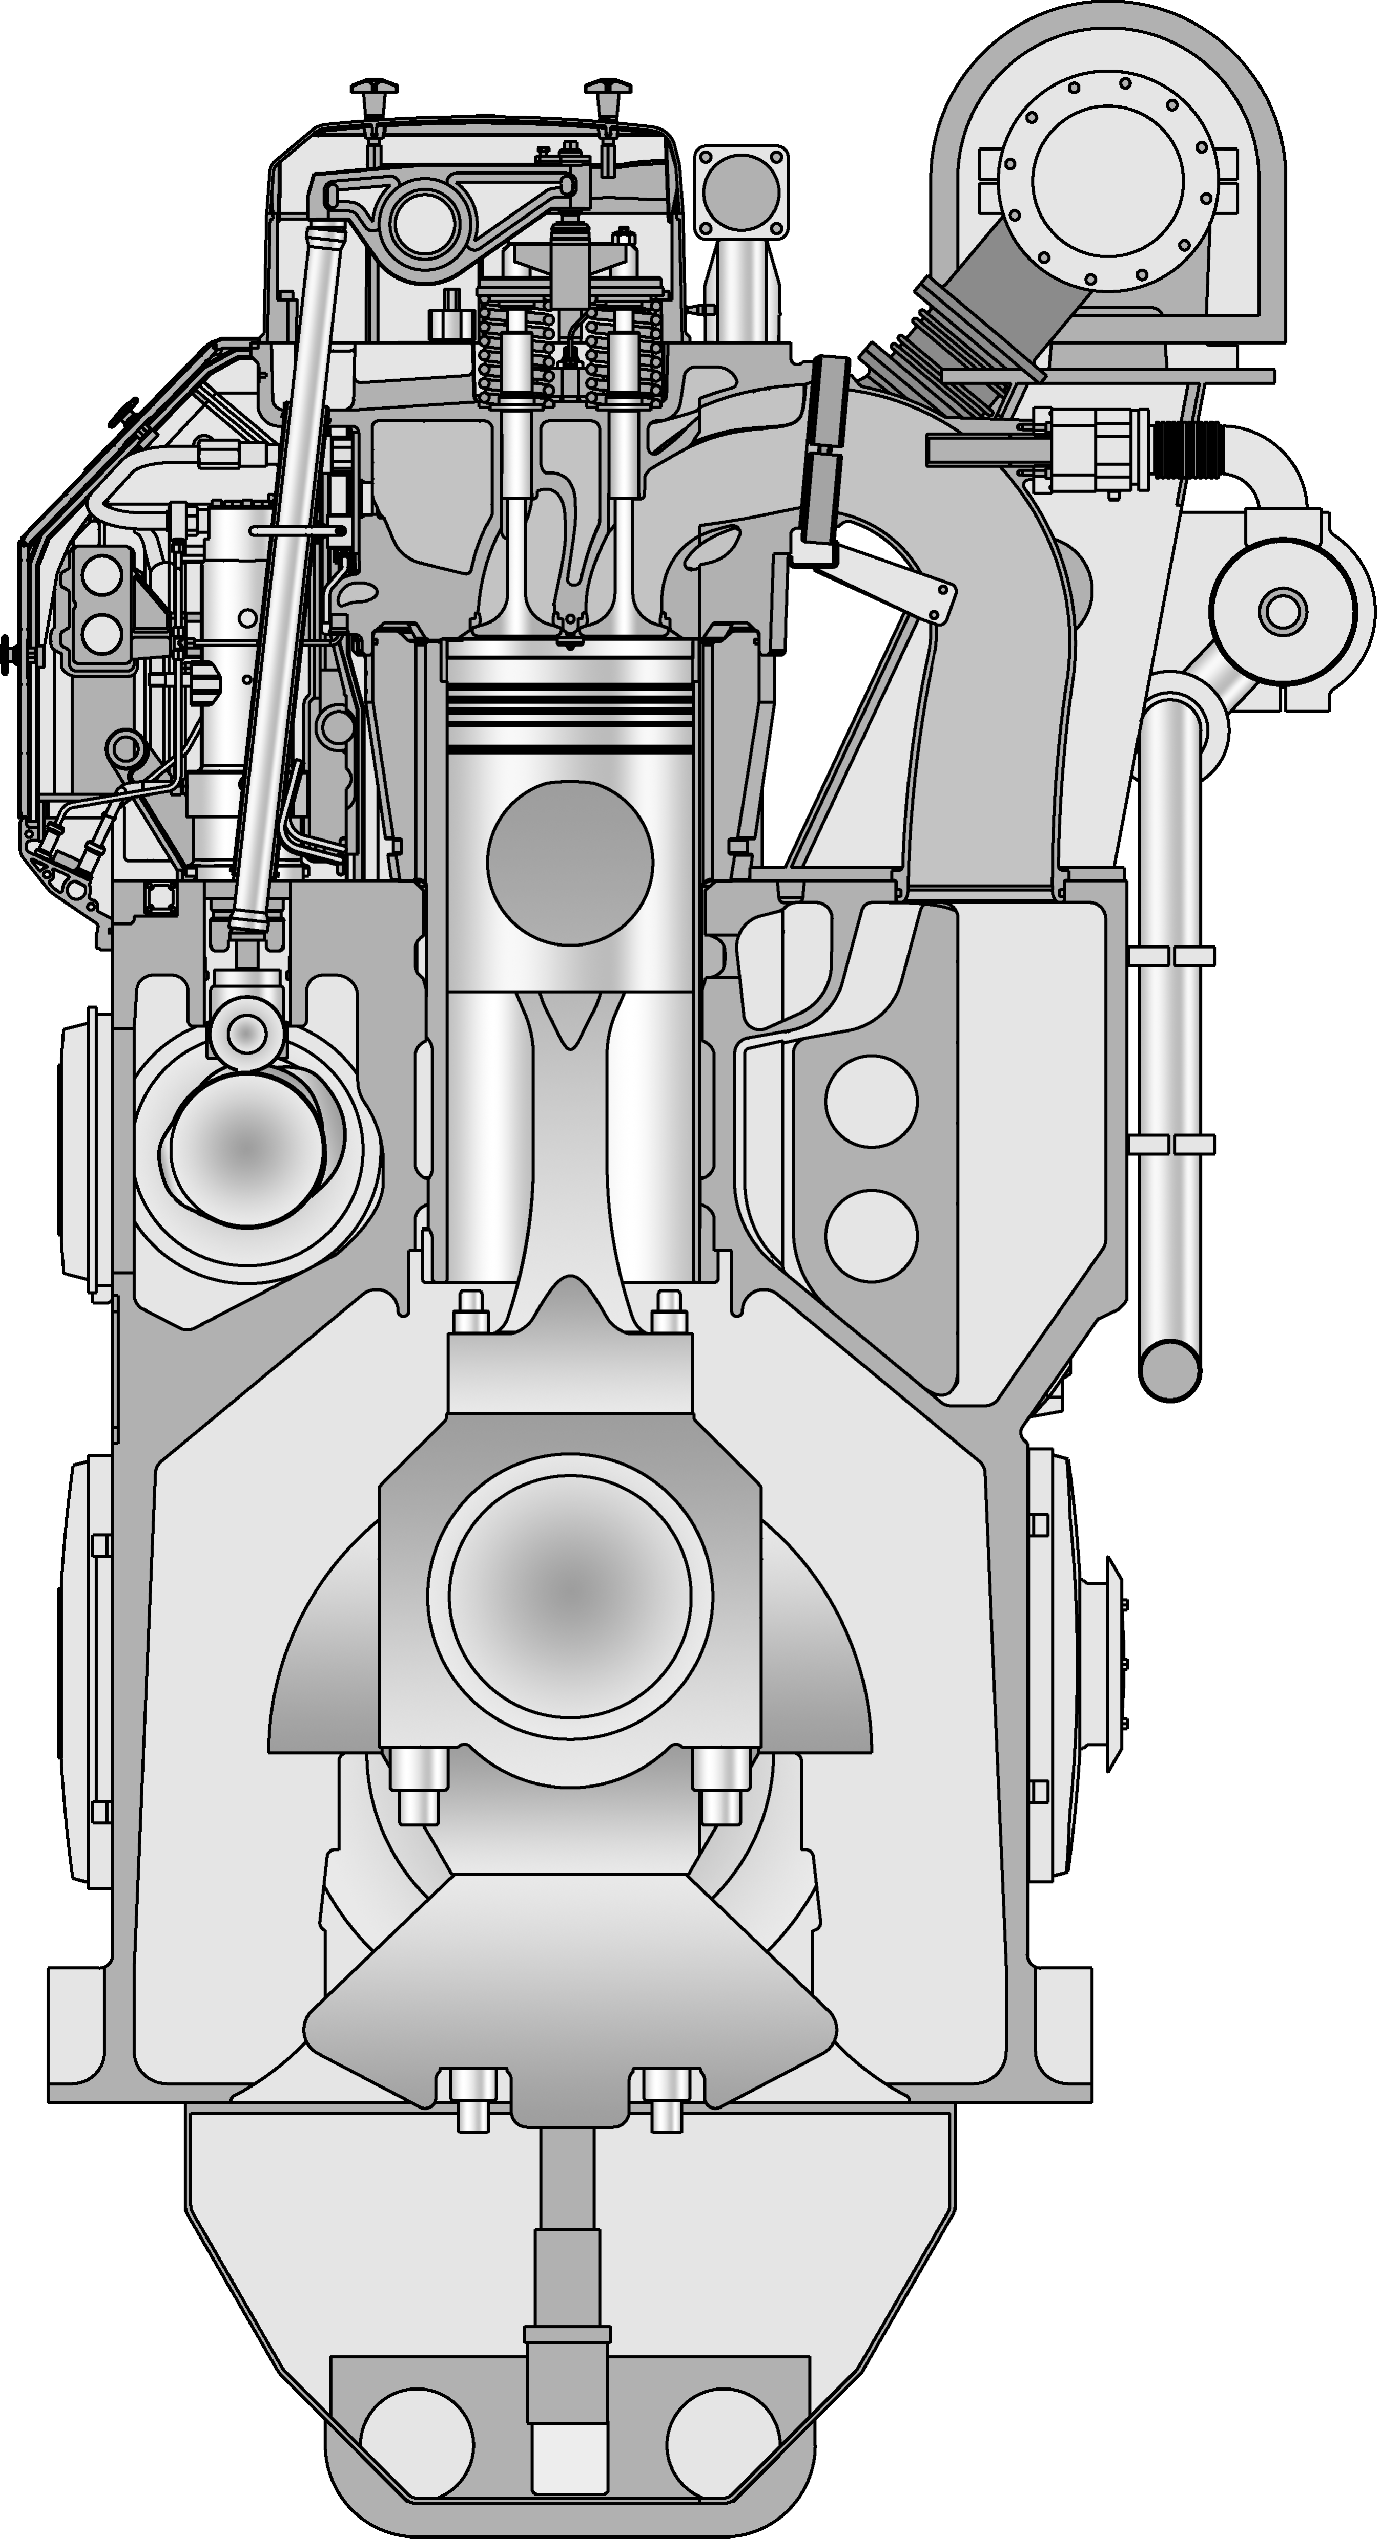
\includegraphics[scale=0.2]{img/8L50DF}
			\end{figure}


\vfill
~
\flushright{Cyrille Reggio} 
\flushright{2017}
\cleardoublepage

%%%%%%%%%%%%%%%%%%%%%%%%%%%%%%%%%%%%%%%%%%%%%%%%%%%%%
\flushleft
\justifying
\cleardoublepage
\pagestyle{fancy}
\section{Pilot Sheet}
\begin{table}[htbp]
\begin{tabular}{|l|r|}
\hline
DeadWeight & 55.000 tpl \\ \hline
Length & 218 m \\ \hline
Breadth & 31,8 m \\ \hline
Speed & 23 nds \\ \hline
Propulsive Power & 21000 kW \\ \hline
Number of Electric Propulsion Engine & 2 \\ \hline
Generator & 4 x Wärtsilä 8L50DF (4 x 7,600 kW) \\ \hline
Delivered Voltage & 6,6kV \\ \hline
Mainbus Voltage & 4x400V \\ \hline
Bow thruster & 2 \\ \hline
Stern Thruster & 1 \\ \hline
\end{tabular}
\caption{Main Caracteristics}
\label{}
\end{table}


\subsection{Dual Fuel Engines}

\subsubsection{Wartsila 8L50DF}

\begin{itemize}
 \item Power 7600 kW @ 500 rpm
 \item Bore 500 mm
 \item 8 cylindres en ligne
 \item Air cooler
 \item 2 turbochargers 
 \item gas mode / DO-HFO / backup (no PI)
\end{itemize}
% \section{Objectifs}
%
% \subsection{Déroulé de la séance}
%
% La séance s'articule autour de la mise en service du navire à a partir d'une situation initiale ou le navire est en arrêt technique et doit reprendre les opérations (Cold Ship). Les étapes seront donc :
% \begin{enumerate}
%  \item Démarrage d'un groupe au DO,
%  \item Alimentation électrique du navire,
%  \item Mise en froid de la cuve,
%  \item Chargement GNL,
%  \item Passage au gaz d'un groupe,
%  \item Mise en service de la propulsion,
%  \item Passage des commandes en passerelle.
%  
% \end{enumerate}
%L'accent sera mis néanmoins sur les particularités du système GNL;

%\section{Systèmes abordés }
%
% Les systèmes représentés par le simulateur DFDE sont les suivants :
% 
% \begin{itemize}
%  \item Système de contrôle IAS (Integrated Automation System)
%  \begin{itemize}
%        \item Gestion des alarmes,
%        \item Gestion de la puissance électrique,
%        \item Système propulsif.
%        \item Gestion des GE Dual Fuel,
%  \end{itemize}
%  \end{itemize}
%    
%\begin{itemize}
%    \item Système de contrôle des opérations GNL (Control System)
%    \begin{itemize}
%        \item Avitaillement GNL (camion, barge ou pipe),
%        \item Monitoring des opérations,
%        \item Qualité du gaz,
%        \item Système ESD,
%    \item Stockage GNL
%    \end{itemize}
%    \item Opérations sur le gaz avant alimentation des groupes.
% \end{itemize}
%
 \section{Starting the simulator}
\begin{enumerate}
 \item Launch \emph{DEDF42-CF},
 \item Choose initial condition "cold ship",
\end{enumerate}

Run simulation with "F1", most common keyboard shortcuts are listed down below : 
 

    \begin{table}[htbp]
    \centering
    \footnotesize
        \begin{tabular}{|l|l|}
        \hline
        Raccourci & Fonction \\ \hline
        F1 & Run \\ \hline
        F2 & Freeze \\ \hline
        F3 & Stop \\ \hline
        Shift+F6 & Initial condition \\ \hline
        Home & main page \\ \hline
        Pg Up & page increment \\ \hline
        Pg Down & page decrement \\ \hline
        F12 & Ack buzzer \\ \hline
        \end{tabular}
    \label{Raccourcis clavier}
    \caption{Shortcuts}
    \end{table}



%%%%%%%%%%%%%%%%%%%%%%%%%%%%%%%%%%%%%%%
\section{Global procedure from Cold Ship to underway}

\subsection{Global sequence}

\begin{table}[htbp]
\scriptsize
\begin{tabular}{||c||l||l||}
\hline
Etape & Action & Page  \\ \hline
1 &  Line up for MDO from MDO Service tank to DGs via the Emergency Fuel Feed Pump & (MD455 \& 460) \\ \hline
2 &  Line up DG LO system & (MD 305 \& 310) \\ \hline
3 &  Line up DG cooling water system& (MD405-410) \\ \hline
4 &  Start DG from local stand and connect it to main switchboard & (MD205-220) and MD105 \\ 
& Note! Connect electrical consumers to main switchboard to achive heating from DGs. & \\ \hline
6 &  Line up for normal fuel supply & (MD460) \\ \hline
7 &  Prepare ventilation & \\ \hline
8 &  Prepare LNG supplier for bunkering (truck, ship or terminal) (MD480) &\\ \hline
9 &  Prepare vessel for bunkering &(MD510 \& 755) \\ \hline
10 &  Line up for heating of LNG & (MD515) \\ \hline
11 &  Prepare Gas Supply to DGs & \\ \hline
12 &  DO/HFO-Gas Change Over &\\ \hline
13 &  Line up and start up next Diesel Engine, start on Gas and connect to main switch board &\\ \hline
14 &  Prepare for start up of propulsion from engine control room &\\ \hline
15 &  Transfer control position to bridge &\\ \hline
16 & Ready for Departure &\\ \hline
\end{tabular}
\caption{Global sequence}
\label{}
\end{table}

%%%%%%%%%%%%%%%%%%%%%%%%%%%%%%%%%%%%%%%%%\
\subsection{Bunkering}

\subsubsection{Equipements}

Viking Grace is operated with two type C tanks for a total volume of $400 ~m^3$. Tank pressure is $5~bar$ at a temperature of $-127 \degree C$. Two nitrogen tanks are used for inerting circuits for bunkering, gas delivery to engine and expansion tank for HTFW circuit. Pressure is regulated to $8~bar$.
\image{BS}{LNG Bunkering System}{0.6}

Each tank is equiped with a drop line for bunkering in liquid phase and a spray line for the regulation of the tank pressure :

\begin{itemize}
 \item Vaporising liquid drops for tank cooling in cooling down operation,
 \item Tank pressure control when bunkering,
\end{itemize}

Liquid and vapor line for tanks are designed to be connected to ensure operation on both tanks at the same time.

\subsection{LNG feeding}

Gas pressure delivered to GVU is $6.3~ bar$. At the admission pipe of the engine, delivered pressure is $2.3~ bar$ at $34,1 \degree C$.

\image{LNGPAC}{LNG pac}{0.6}
%%%%%%%%%%%%%%%%%%%%%%%%%%%%%%%%%%%%%%%%%%%%%%
\subsection{Evaporators}

\subsubsection{Pressure Build Up Evaporator}

\emph{Pressure Build Up Evaporator} function is to build up tank pressure at $5,3~bar$, gas is vaporised with the LTFW. Heat exchange is done by using a silicone gel (Syltherm).\\

Pressure build-up has to be done : 
\begin{itemize}
    \item After bunkering operation (Initial Build Up),
    \item when ship is underway to face the gaz consumption,
\end{itemize}
Produced vapor returns to the tank.



\subsubsection{Main Gas Evaporator}


\emph{Main Gas Evaporator} role is to regulate pressure delivered to the engine. Feeding of the evaporator is in liquid phase, pressure is regulated by regulating valve in and out of the evaporator.

\subsubsection{Gas Heater}

\emph{Gas Heater} role is to ensure precision for temperature and pressure delivered to the engine. Gas heater has its own FW feeding.

Pressure of the evaporator (PBE, GVE) is regulates with (V96) valve. A portion of the main flow is then redirected to the Gas Heater. While underway, the position of the valve is 40\%.\\



\subsection{Safety valves}

Les soupapes de sûretés sont placés à différents endroits du circuit, leur pression de tarage est de $9~bar$. Leur refoulement est effectué au mât de dégazage.

\section{Shutdown}

Il est prévu plusieurs situations de Shutdown :
\begin{itemize}
 \item \textbf{TAS} Tank Shutdown : En cas de défaut du circuit \emph{LNG PAC}, les évents s'ouvrent afin de dé-pressuriser le tuyautage et les vannes automatiques fermées. Un système de retour du gaz en phase liquide séquencé à la citerne permet de ne vaporiser que le minimum de gaz.  
 \item \textbf{CB} Close Bunkering : Lors de la fin de l'opération d'approvisionnement, par fermeture des vannes bunkering ou en cas de niveau haut ou de pression haute dans la citerne, 
 \item \textbf{BS} Bunkering Shutdown : Les vannes d'approvisionnement si elles sont fermées en manuel pendant l'opération provoquent un shutdown.
 \item \textbf{ELS} Engine Line Shutdown : En cas d'incident sur le circuit d'alimentation gaz, les vannes d'entrée et de sortie au MGE, et la vanne d'interconnexion sont fermées, le signal de shutdown est envoyé à la GVU.
 
\end{itemize}

%\subsection{Ventilation}
%
%La ventilation est pilotable par l'IAS et dispose de capteurs $CH_4$ et $O_2$;
%
\subsection{Détection gaz et ESD}

La détection est basée sur la détection de gaz et d'oxygène. Une pré-alarme et une alarme dont le seuil peut être configuré dans le \emph{Gas Detector Panel}. 


\section{ Control System (LNG Monitor)
}

Le système de contrôle automatise largement les procédures liées au circuit gaz et permet le contrôle et suivi des opérations.

\image{ControlSystem}{Code couleur système de contrôle gaz}{}

\subsubsection{Control Box Command}

Elle permet d'effectuer les opérations sur le combustible et d'en contrôler le déroulement.  
%
\image{stoTank}{Disposition Storage tank}{}
%
Les tableaux ci-dessous illustrent chaque séquence en automatique des différents éléments du circuit.

\imcac{VRL.eps}{LIL.eps}{0.5}
\imcac{LBL.eps}{PBE.eps}{0.5}
\imcac{BC.eps}{MGE.eps}{0.5}
\imcac{EL.eps}{GIL.eps}{0.5}
\vfill

%%%%%%%%%%%%%%%%%%%%%%%%%%%%%%%%%%%%%%

\cleardoublepage



%%%%%%%%%%%%%%%%%%%%%%%%%%%%%%%%%%%%%%%%%%%%
\begin{center}

\begin{tabular}{|p{0.6\linewidth} |}
    \hline\\
    {\large{
    \makecell{Procédure démarrage groupe\\
   Alimentation électrique
    }
    }}
    \\\\\hline
    \end{tabular} 
\end{center}
\cfoot{I}

%Prerequisite: Cooling water, lubrication oil and fuel oil lined up and ready for operation.
%Note : Start air is always available.
%

\textbf{ Pré-requis}
Les circuits suivants doivent être disposés :
(Vannes ouvertes, pompes auxiliaires démarrées)

\begin{enumerate}
 \item EDBT
 \item Huile
 \item DO (la pompe de secours DO fonctionne à l'air comprimé Emergency Fuel Feed Pump)
\end{enumerate}

\emph{Nota : L'air comprimé est toujours disponible.}\\
Avant de démarrer un groupe, il faut le passer en mode DO/HFO, en effet en mode back-up (par défaut) il est impossible de passer en mode gaz sans le stopper.\\
%\begin{enumerate}
% \item Acknowledge any alarm and check for any start block, 
% \item Open turbocharger inlet flap %(ouvrir le volet de la TS),
% \item Check that turning gear is out
% \item Blow through engine by putting control mode selector to “BLOW”
% \item Start engine locally by setting selector to local and push start button
% \item When confirmed that engine is running properly, put the engine to remote control.
%\end{enumerate}
%
\textbf{Démarrage :}
\begin{enumerate}[resume]
 \item Ouvrir le volet (flap),
 \item Effectuer un virage électrique puis débrayer le vireur (turning gear),
 \item Effectuer un virage à l'air (Blow),
 \item Repasser en local,
 \item Acquiter les alarmes,
 \item Passer en mode run sur le sélecteur,
 \item Démarrer et observer la montée en température des échappements, 
 \item Si les paramètres sont corrects, passer le groupe en remote.
\end{enumerate}
Nous pouvons alors disposer l'alimentation électrique sur les barres principales et alimenter les consommateurs.
\begin{enumerate}[resume]
 \item Connecter le disjoncteur principal,
 \item Alimenter le jeu complet de barres,
 \item Alimenter les consommateurs.
\end{enumerate}
Il est possible maintenant de disposer les pompes principales et auxiliaires des circuits ED et huile en automatique.\\
Passer le DG1 en priorité 1 / auto / alone on bus\\
Stopper la pompe MDO à air.

\subsection*{Attention :}

La régulation de température ED ne peut être passée en automatique \textbf{que sur l'IAS}. Il faut :
\begin{itemize}
 \item Passer les vannes trois voies de régulation en remote sur le circuit, 
 \item Puis sur l'IAS dans la page FW Cooling System, passer les vannes correspondantes en auto. 
\end{itemize}
 La vanne prend alors une couleur orange pour signaler qu'elle régule.

\newpage
\cfoot{II}
\begin{center}

\begin{tabular}{|p{0.6\linewidth} |}
    \hline\\
    {\large{
    \makecell{Procédure d'approvisionnement GNL \\ 
    Citernes à température ambiante
    }
    }}
    \\\\\hline
    \end{tabular} 
\end{center}

Dans cet exemple nous utiliserons le camion et l'approvisionnement sera fait sur la citerne babord.\\
Les phases suivantes doivent être suivies :
\subsection*{Préparatifs côté camion}
Un test d'étanchéité des vannes de la ligne liquide et vapeur doit être effectué. 
\begin{enumerate}
 \item Inerter les lignes liquide et vapeur,
 \item Stopper l'inertage et vérifier l'absence de fuites,
 \item Mettre les lignes à l'air,
 \item Fermer les vannes des lignes liquides et vapeur.
\end{enumerate}
 Quand le navire est prêt (joint plein déposé), connecter le bras de chargement. \\
 Prévenir le bord qu'un test ESD doit être conduit.\\
 
 \emph{Noter que le bord peut procéder à l'inertage du camion et que le camion peut procéder à l'inertage du bord.}
 \subsection*{Préparatifs côté bord}
Les opérations seront conduite à partir de la page \og LNG Monitor System \fg.
\\
\textbf{Inertage}
\begin{enumerate}
 \item Ouvrir la bride côté navire et brancher le flexible du camion,
 \item Mise en place du rideau d'eau,
 %\item Test de fuite
 \item Inertage à l'azote, lors de cette opération, la commande Inert devra être envoyée deux fois pour :
 \begin{enumerate}
  \item Dépressuriser
  \item Inerter
 \end{enumerate}

    \emph{Dans les opérations d'inertage, attention à ne pas \og activer~\fg !}\\
Les opérations seront conduites en \gui{automatique} sélectionner \gui{All in auto}. L'inertage se conduit de la citerne vers la connexion.
    \begin{itemize}
        \item Inertage des Bottom Connection (BC)
        \item Inertage des Liquid Interconnection Line (LIL)
        \item Inertage de la Port Liquid Bunker Line (LBL)
    \end{itemize}
 \item Ouvrir (activate) la Bottom Connection 1 (V20),
 \item Ouvrir (activate) la Liquid Interconnection Line (select tank 1 / activate) (V01),
 \item Ouvrir la rampe haute Top Spray (LIL) (V02),
 \item Activer la Liquid Bunker Line (V37),
 \item Ouvrir en manu la vanne de tête (V57)
 \item Activer et tester l'ESD (la vanne de la LIL (V57)  doit se fermer)
\end{enumerate}
Un test de fuite (Leak Test) doit être maintenant effectué sur la bride de chargement, pour cela :\\
\begin{enumerate}
\item Mettre en pression à l'azote (8 bar) la ligne entre le camion et la vanne de tête (V57), 
 
 \item Ouvrir la vanne d'alimentation d'azote et la vanne (V58 MD510),
 \item Fermer la vanne d'alimentation et vérifier l'absence de fuite (pression à 8 bar),
 \item mettre à l'air par l'évent (V10 MD510),
 \item fermer l'évent.
\end{enumerate}
\subsection*{Mise en froid des citernes}

\begin{enumerate}[resume]
 \item Ouvrir la vanne manuelle d'isolement (V56 MD510)
 \item Commander la mise en froid en vapeur par la ligne liquide du camion à débit faible ($5~m^3/h $), sélectionner \emph{VAPOUR} puis \emph{ON}. La température 
 \item Démarrage par la LBL de la control box (V57),
 \item Descente en froid jusqu'à $-60 \degree C$ du tuyautage et de la citerne,
 \item Ouverture ligne liquide et montée progressive jusqu'à $400~m^3/h$,
 \item Vaporisation (spray) en auto (LIL), baisser la consigne de pression (Setpoint Bunkering) à $1,0~bar$, cela a pour effet de garder la cuve la plus froide possible en jouant sur la vaporisation. 
\end{enumerate}
\subsection*{Début de l'approvisionnement en GNL}
Si la contre pression augmente dans la citerne, ouvrir la ligne de retour vapeur. 

\subsection*{Finalisation}
\begin{enumerate}
 \item à 85\%, demander au camion de chasser le liquide à la vapeur (1 minute à $5~m^3/h$),
 \item Stopper l'approvisionnement par la Control Box (Stop LBL) (V57),
 \item Désactiver (V37) et purger la BL (V35, V36), pour cela il faut ouvrir sur le spray de la (LBL),
 \item inerter la ligne liquide (inert LBL) (V55, V36, V38) (2 fois),
 \item purger la LIL par la spray line (V55) et l'inerter (V05) (2 fois),
 \item Repasser la consigne Setpoint Bunkering à $5~bar$.
\end{enumerate}

Déconnecter la bride, \textbf{opération d'approvisionnement terminée}.
\vfill
\newpage

%
%%%%%%%%%%%%%%%%%%%%%%%%%%%%%%%%%%%%%%%%%%%%
\cfoot{}
\cfoot{III}
\begin{center}

\begin{tabular}{|p{0.6\linewidth} |}
    \hline\\
    {\large{
    \makecell{Procédure d'approvisionnement GNL \\ 
    Citernes froides
    }
    }}
    \\\\\hline
    \end{tabular} 
\end{center}
Cette procédure s'applique la plupart du temps, en effet, si un talon de GNL existe dans la citerne elle est considérée comme froide.\\
%\subsection{Situation Tank 2 cooled}

\begin{enumerate}
 \item Établir la connexion avec le terminal, dès que la connexion est 
établie, l'ESD est connectée,
 \item Tester l'ESD, (V57)
 \item Vérifier l'étanchéité de la connexion,
 \item Activer la BC
 \item Activer la LIL depuis la control box en activant : \og tanks 
Activate~\fg,
 \item depuis la LBL control box sélectionner \og cool~\fg puis \og activate~\fg et enfin \gui{start}
\end{enumerate}

\emph{Les vannes manuelles doivent être disposées correctement pour pouvoir 
autoriser l'ouverture de la vanne commandée.}

\begin{enumerate}[resume]
 \item Activer le retour vapeur (V03 et V51)
 \item Procéder à l'ouverture coté barge ou terminal de la vanne liquide et vapeur, attendre que la pression soit de $4,5~bar$,
 \item Démarrer l'opération d'approvisionnement (de $50~m^3/h$ jusqu'à 
$400~m^3/h$)
 \item À $85~\%$, commencer à réduire le débit liquide et demander à la barge d'ouvrir la ligne vapeur (vapor bunkering) afin de préssuriser les lignes pour pousser le liquide,
 \item Quand il n'y a plus de débit liquide, attendre $30~sec$ pour vider les lignes puis stopper l'opération d'approvisionnement (STOP et deactivate depuis la LBL control box), \item Purger la LBL (drain),
 \item Purger la LBL,
 \item Inerter LIL,
 \item Inerter LBL,
\end{enumerate}
 Il faut procéder maintenant au débranchement du flexible :
 
\begin{enumerate}[resume]
 \item Procéder à l'inertage avec l'azote du bord par la (V58), 
 \item Quand la pression d'azote atteint les $8~bar$, purger la ligne liquide 
vers la barge,
 \item Fermer la vanne (V58), ouvrir l'évent de la ligne liquide de la barge,
 \item Quand la pression est nulle, fermer l'évent vers la barge,
 \item Fermer la partie liquide coté barge.
\end{enumerate}
Afin de ne pas envoyer de gaz à l'atmosphère lors de la déconnexion, il faut 
procéder à l'inertage de la VRL.

\begin{itemize}[resume]
 \item Informer la barge de l'ouverture de l'évent de la VRL,
 \item Mettre en manuel la VRL,
 \item Fermer le retour vapeur (V03),
 \item Ouvrir sur l'azote (V04) pour procéder à l'inertage vers la barge,
 \item Quand l'inertage est terminer, fermer les vannes et repasser la VRL en 
auto,
 \item Désactiver et inerter la VRL depuis la control box,
 \item purge la VRL vers la barge et quand la pression est nulle, stopper et 
isoler l'inertage,
 \item Quand le flexible est dépressurisé, fermer la vanne manuelle 
d'alimentation (V56),
 \item Débrancher le flexible et placer la bride pleine,
 \item Purger la ligne en ouvrant plusieurs fois la vanne (V56) et (V58)
 \item Inerter en ouvrant la vanne (V10)
 
\end{itemize}

\textbf{Fin de l'opération d'approvisionnement.}


\vfill

\newpage

\cfoot{}
\cfoot{IV}
\begin{center}

\begin{tabular}{|p{0.6\linewidth} |}
    \hline\\
    {\large{
    \makecell{Passage des moteurs au gaz}
    }}
    \\\\\hline
    \end{tabular} 
\end{center}
\section*{Disposition GNL}

Il faut disposer le système de réchauffage des évaporateurs;
\begin{enumerate}
 \item Vérifier le niveau de la caisse à expansion et disposer le détendeur 1,5 bar d'azote,
 \item Disposer le circuit d'eau, régulation en automatique,
 \item Disposer l'air conditionné HVAC,
 \item Démarrer les pompes.
\end{enumerate}
Disposition de l'alimentation en gaz des moteurs.
\begin{enumerate}[resume]
 \item Activer la BC, si elle a été dépressurisée, elle doit d'abord être inertée,
 \item Activer le Pressure Build Evaporator la consigne de pression doit être de $5~bar$,
 \item Activer la Engine Line,
 \item Quand la pression de la citerne est correcte, activer le Main Gas Evaporator, l'inerter si besoin,
 \end{enumerate}
La connexion Gas Interconnection Line peut être activée, il faut néanmoins :
\begin{itemize}
 \item Avoir un MGE en service,
 \item Que l'autre MGE soit stoppé mais pressurisé.
\end{itemize}
Le gaz est disposé.
\section*{Passage des moteurs au gaz}
\begin{enumerate}
 \item La ventilation du compartiment moteur doit être démarrée puis passée en auto 
 \item La vanne manuelle d'alimentation de la GVU (V051) doit être disposée,
 \item La GVU control en auto,
 \item Le gas Mode est disponible.
\end{enumerate}
Il est possible de démarrer directement au gaz.
\newpage
%
%\cfoot{}
%\cfoot{V}
%\begin{center}
%
%\begin{tabular}{|p{0.6\linewidth} |}
%    \hline\\
%    {\large{
%    \makecell{Inertage des tanks}
%    }}
%    \\\\\hline
%    \end{tabular} 
%\end{center}

\end{document}



%00:42:08
%23, 51, 84
